\chapter{Architectural Views for Your Suggestions to Improve the Existing System} \label{suggest}


\section{Context View}

\subsection{Stakeholders’ uses of this view}
The Context View is vital for stakeholders to understand FarmBot’s integration with external systems, emphasizing enhanced functionality:
\begin{itemize}
    \item \textbf{Hobbyist Gardeners and Professional Farmers:} These users see how FarmBot’s integration with services like the OpenWeather API and the mobile application optimizes farming based on real-time data, facilitating remote management.
    \item \textbf{Educators:} They use the Context View to show students FarmBot’s connectivity to technologies such as the OpenWeather API and mobile apps, illustrating practical applications of integrated agricultural technology.
    \item \textbf{Researchers:} Researchers explore how external data sources like the OpenWeather API influence FarmBot’s functionality, with the mobile app providing essential real-time control and data access for experiments.
    \item \textbf{Software Developers:} Developers assess how the mobile application and external APIs like OpenWeather interact with FarmBot’s core systems, crucial for developing responsive applications.
    \item \textbf{System Administrators:} Admins monitor FarmBot’s performance with external services including the OpenWeather API and mobile app, ensuring reliability and a seamless user experience.
    \item \textbf{Open-Source Contributors and Community Members:} Contributors identify opportunities to enhance FarmBot’s capabilities, focusing on the mobile application and third-party service integrations to improve functionality.
\end{itemize}
Each stakeholder group uses the Context View to effectively support and utilize the FarmBot system, leveraging its connections with external technologies.

\subsection{Context Diagram}
\begin{figure}[htbp]
    \centering
    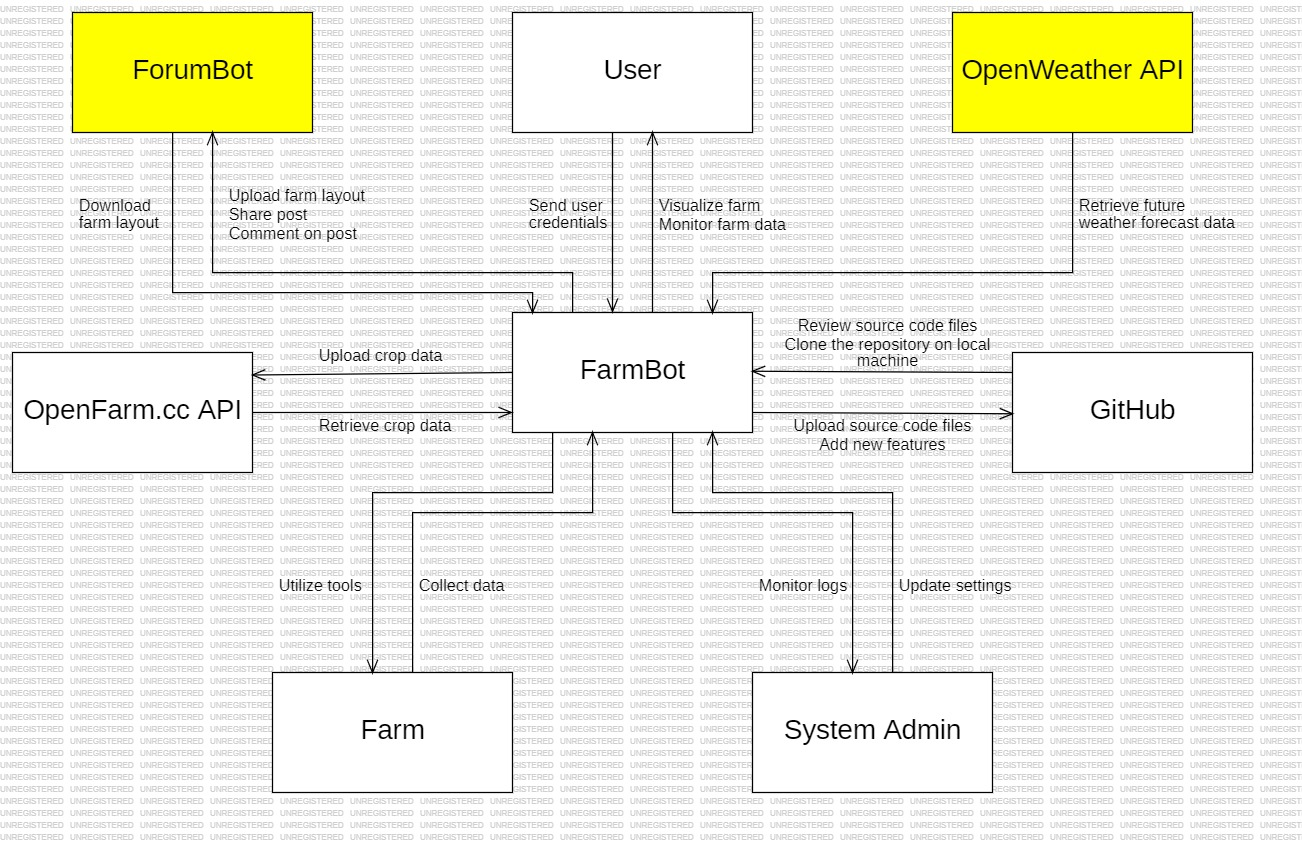
\includegraphics[width=1\linewidth]{Figures/improved_context_diagram.jpg}
    \caption{Context Diagram for the Improved System}
    \label{ContextImproved}
\end{figure}
\newpage
The updated Context Diagram of FarmBot reflects the integration of new features and external interfaces that further enhance its capabilities for autonomous agricultural management. Here’s how the system now interacts with new components:
\begin{itemize}
    \item \textbf{ForumBot:} A new addition that facilitates user interaction within the FarmBot community by enabling discussions, knowledge exchange, and the sharing of custom farm layouts and strategies, fostering a collaborative user environment.
    \item \textbf{OpenWeather API:} Newly integrated to provide real-time weather data directly to FarmBot, allowing the system to make immediate adjustments to farming operations based on current weather conditions, enhancing responsiveness to environmental factors.
\end{itemize}
The revised context diagram illustrates FarmBot’s evolution into a more connected, responsive, and user-focused system. These enhancements not only improve FarmBot's operational efficiency but also enrich the user experience and community engagement, ensuring that the system remains at the forefront of technology-driven sustainable agriculture.

\newpage
\subsection{External Interfaces}
\begin{figure}[htbp]
    \centering
    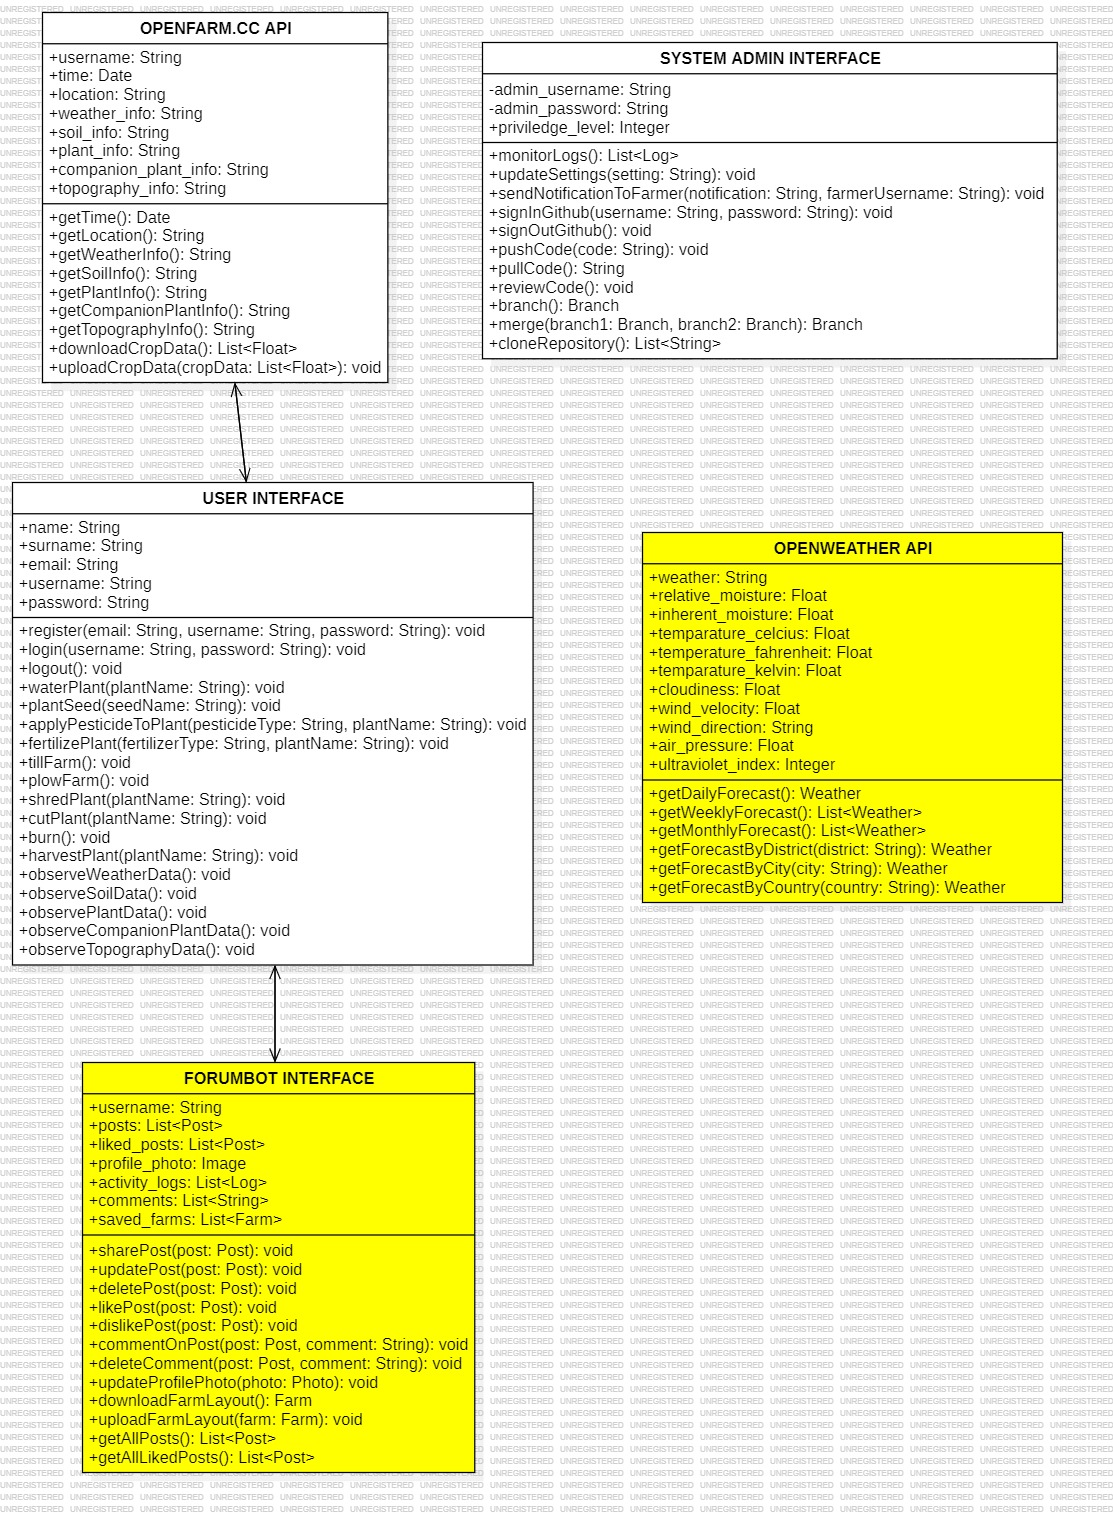
\includegraphics[width=0.7\linewidth]{Figures/improved_external_interfaces.jpg}
    \caption{External Interfaces Class Diagram for the Improved System}
    \label{ExternalImproved}
\end{figure}
\newpage
In the enhanced architecture of the FarmBot system, significant developments in the external interfaces include the addition of the OpenWeather API and the ForumBot Interface, which broaden the capabilities of data interaction and community engagement:
\begin{itemize}
    \item \textbf{ForumBot Interface:}
        \begin{itemize}
            \item \textbf{username:} Unique identifier for a user within the ForumBot community.
            \item \textbf{posts:} A collection of posts made by a user.
            \item \textbf{liked\_posts:} List of posts that the user has liked.
            \item \textbf{profile\_photo:} Image file that represents the user’s profile picture.
            \item \textbf{activity\_logs:} Record of user actions and interactions within the community.
            \item \textbf{comments:} Comments made by the user on various posts.
            \item \textbf{saved\_farms:} Collection of farm layouts or strategies that the user has saved for future reference.
            \item \textbf{sharePost}$()$: Allows users to create and share a new post with the community.
            \item \textbf{updatePost}$()$: Method to update a post created by the user.
            \item \textbf{deletePost}$()$: Deletes a specific post made by the user.
            \item \textbf{likePost}$()$: Adds a post to the user’s liked posts list.
            \item \textbf{dislikePost}$()$: Removes a post from the user’s liked posts list.
            \item \textbf{commentOnPost}$()$: Adds a comment to a specific post.
            \item \textbf{deleteComment}$()$: Removes a specific comment made by the user.
            \item \textbf{updateProfilePhoto}$()$: Updates the user's profile photo displayed on the forum.
            \item \textbf{downloadFarmLayout}$()$: Enables users to download a specific farm layout from the community.
            \item \textbf{uploadFarmLayout}$()$: Allows users to upload and share their farm layout with the community.
            \item \textbf{getAllPosts}$()$: Retrieves all posts made within the ForumBot community.
            \item \textbf{getAllLikedPosts}$()$: Retrieves all posts that the user has liked.
        \end{itemize}
    \item \textbf{OpenWeather API:}
        \begin{itemize}
            \item \textbf{weather:} General description of the current weather conditions.
            \item \textbf{relative\_moisture:} The moisture content in the air relative to the temperature.
            \item \textbf{inherent\_moisture:} Absolute moisture content in the air regardless of temperature.
            \item \textbf{temperature\_celsius:} Current temperature in degrees Celsius.
            \item \textbf{temperature\_fahrenheit:} Current temperature in degrees Fahrenheit.
            \item \textbf{temperature\_kelvin:} Current temperature in degrees Kelvin.
            \item \textbf{cloudiness:} Percentage describing the cloud cover.
            \item \textbf{wind\_velocity:} Speed of the wind measured in units per hour.
            \item \textbf{wind\_direction:} Compass direction from which the wind is coming.
            \item \textbf{air\_pressure:} Atmospheric pressure measured in units of pressure (such as pascals or millibars).
            \item \textbf{ultraviolet\_index:} Index indicating the strength of the sun’s ultraviolet radiation at the surface.
            \item \textbf{getDailyForecast}$()$: Retrieves the weather forecast for the current day.
            \item \textbf{getWeeklyForecast}$()$: Retrieves the weather forecast for the current week.
            \item \textbf{getMonthlyForecast}$()$: Retrieves the weather forecast for the current month.
            \item \textbf{getForecastByDistrict}$()$: Provides weather forecasts specific to a district.
            \item \textbf{getForecastByCity}$()$: Provides weather forecasts specific to a city.
            \item \textbf{getForecastByCountry}$()$: Provides weather forecasts specific to a country.
        \end{itemize}
\end{itemize}
The integration of these interfaces into FarmBot’s system enhances the platform's functionality and user engagement. ForumBot enriches the community aspect by allowing more dynamic interactions among users, while the OpenWeather API integrates essential weather data into FarmBot’s operational decisions, ensuring that farming strategies are optimized for current and anticipated environmental conditions. These updates not only enrich the user experience but also bolster FarmBot’s capability as a comprehensive, data-driven agricultural solution.

\newpage
\subsection{Interaction scenarios}
\begin{figure}[htbp]
    \centering
    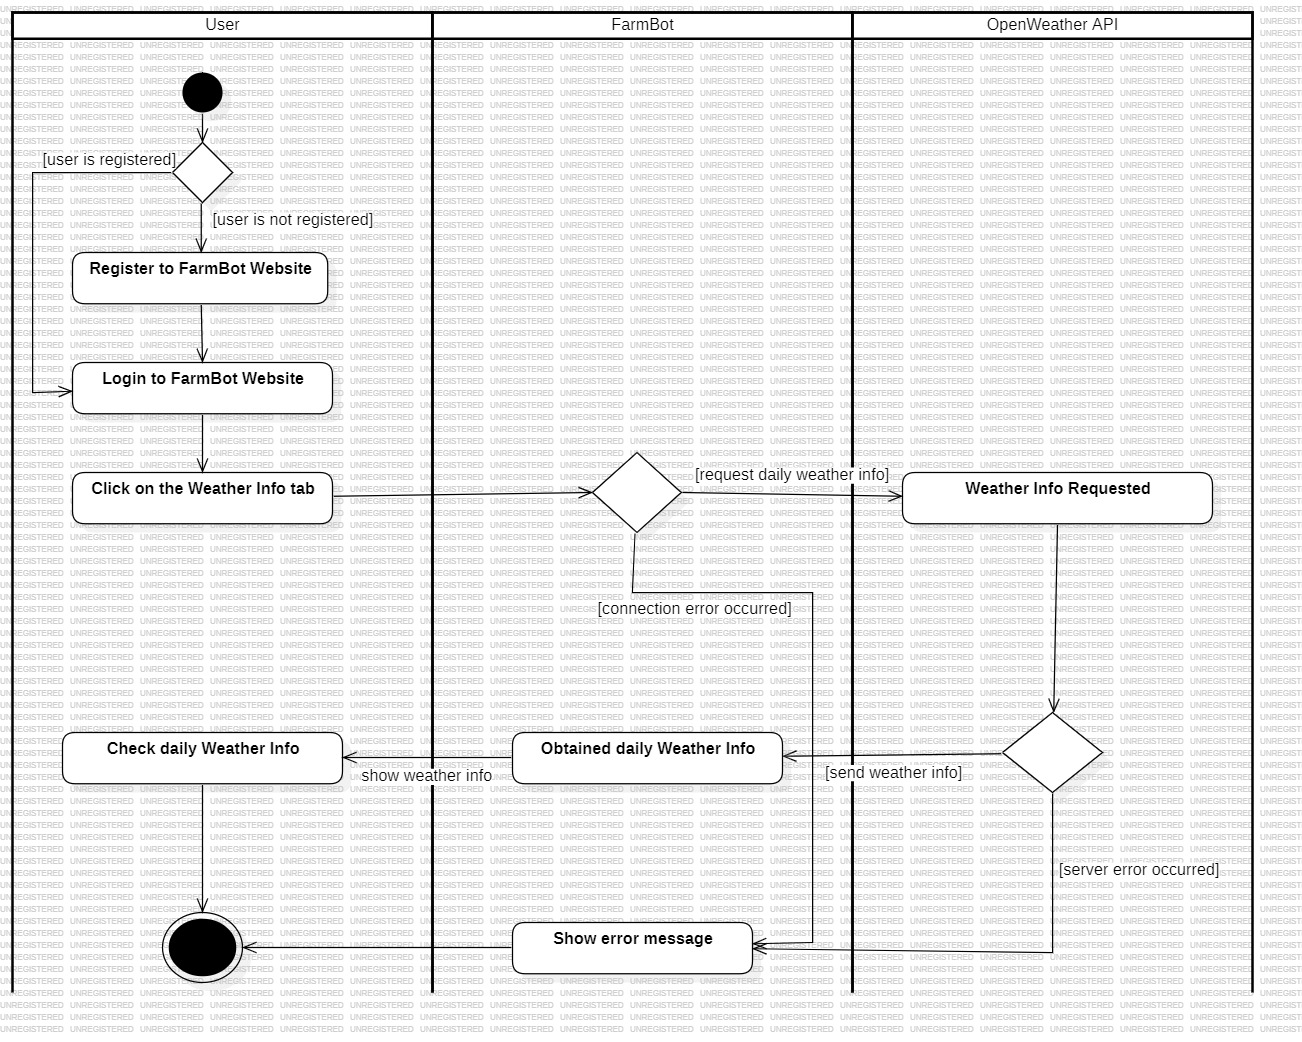
\includegraphics[width=1\linewidth]{Figures/activity3.jpg}
    \caption{Activity Diagram for "Check Daily Wheather Info" Interaction Scenario}
    \label{Activity3}
\end{figure}
\newpage

\section{Functional View}

\subsection{Stakeholders’ uses of this view}
The Functional View offers insights into FarmBot's internal operations, focusing on new features to guide stakeholders in development, usage, and system enhancement:
\begin{itemize}
    \item \textbf{Developers:} Use this view to understand and integrate new features like AI-Driven Weed Identification and the Mobile Application. It helps ensure these functionalities blend seamlessly with FarmBot's existing systems and enhance overall performance.
    \item \textbf{Users (Hobbyist Gardeners, Professional Farmers, Educators):} Access this view to learn how new AI tools improve FarmBot’s efficiency and how the mobile application facilitates remote management, enhancing their daily farming and educational activities.
    \item \textbf{System Admins:} Monitor the performance and reliability of new features, particularly the mobile application, to maintain system integrity and address any issues promptly.
    \item \textbf{Researchers:} Explore how AI-driven features can be applied in agricultural research, particularly for precise disease detection and weed management.
    \item \textbf{Contributors (Open-Source Community Users):} Evaluate how their contributions, such as AI algorithms or mobile app enhancements, fit into FarmBot’s framework and impact its functionality.
\end{itemize}
This streamlined Functional View clarifies the roles of new internal features in FarmBot’s operations, ensuring stakeholders understand how these advancements contribute to the system’s goals of efficiency and user accessibility.

\newpage
\subsection{Component Diagram}
\begin{figure}[htbp]
    \centering
    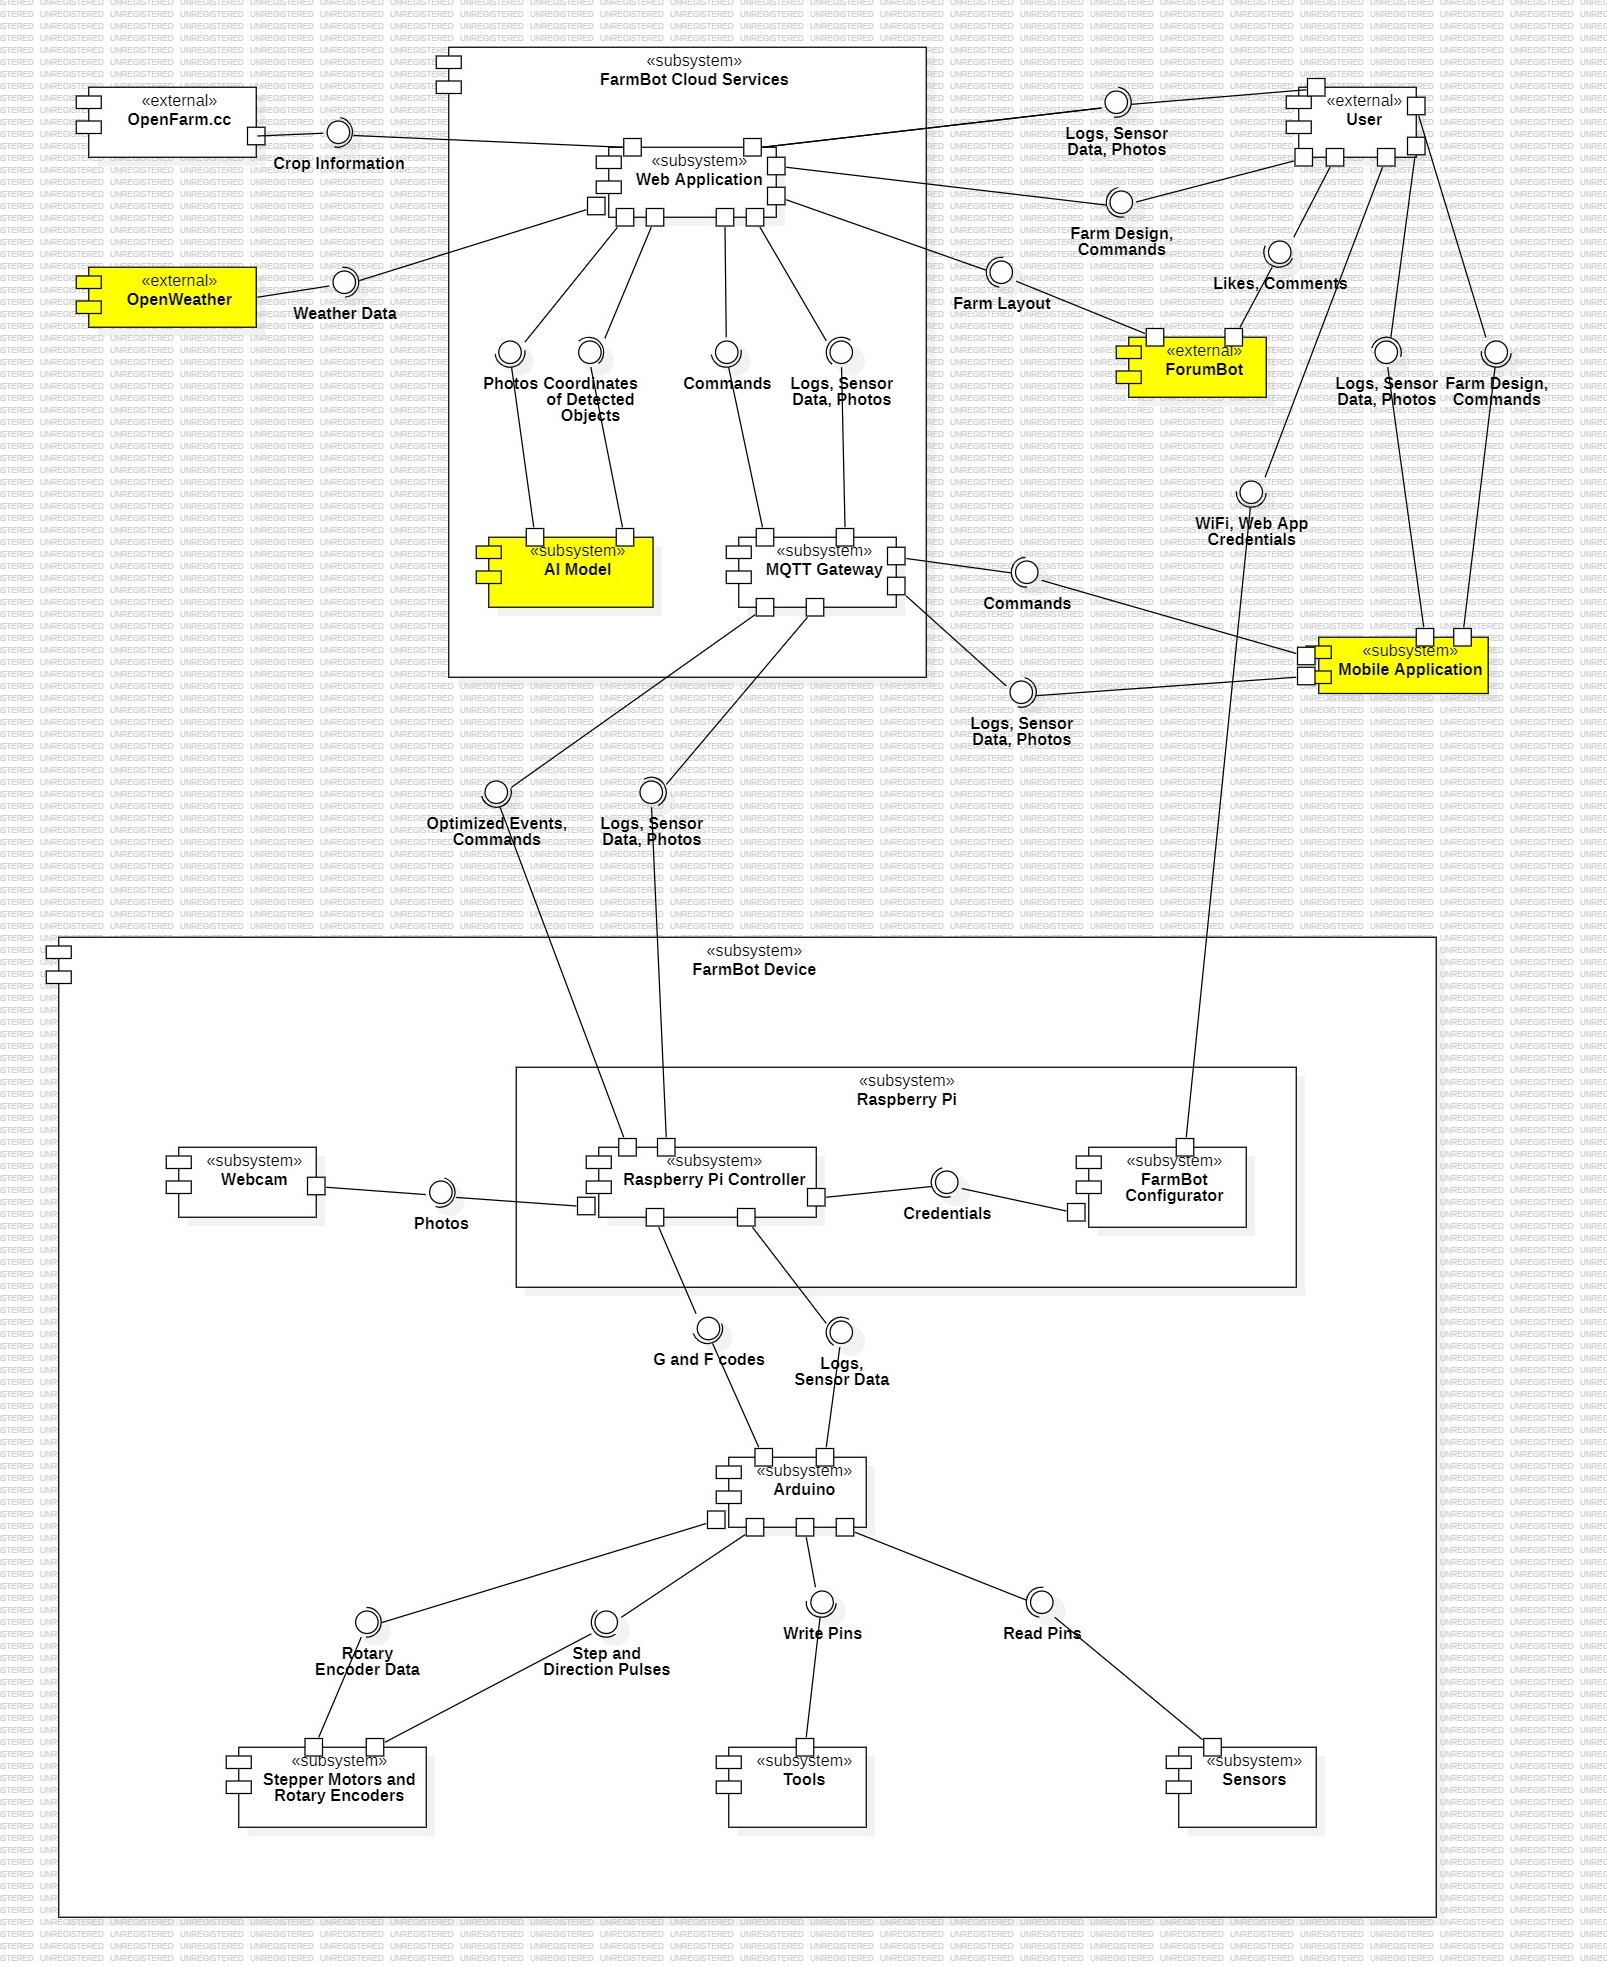
\includegraphics[width=0.8\linewidth]{Figures/improved_component_diagram.jpg}
    \caption{Component Diagram for the Improved System}
    \label{ComponentImproved}
\end{figure}
\newpage
The updated FarmBot system architecture integrates new subsystems and external interfaces, enhancing its capabilities and interaction with external data and user platforms:
\begin{itemize}
    \item \textbf{OpenWeather API:} This integration provides real-time and forecasted weather data crucial for farming decisions. It feeds environmental data directly into the FarmBot Cloud Services, influencing the AI Model's predictive analyses for irrigation and crop management.
    \item \textbf{AI Model:} Positioned within the Cloud Services, the AI Model uses data from OpenWeather and onsite sensors to optimize farming operations. It processes this information to generate actionable insights and commands, which are relayed via the MQTT Gateway to the FarmBot device.
    \item \textbf{ForumBot:} As a new community platform, ForumBot facilitates user interaction by allowing the sharing of farming strategies and insights directly through the Web Application, enhancing community engagement and knowledge exchange.
    \item \textbf{Mobile Application:} This addition extends user interaction capabilities by enabling remote monitoring and management of the FarmBot system via smartphones. It syncs with the Web Application to provide real-time operational control and updates, ensuring a cohesive user experience.
\end{itemize}
These additions make FarmBot more adaptable, responsive, and user-friendly, enhancing its precision farming capabilities and ensuring it remains a leader in automated agricultural technology.

\newpage
\subsection{Internal Interfaces}
\begin{figure}[htbp]
    \centering
    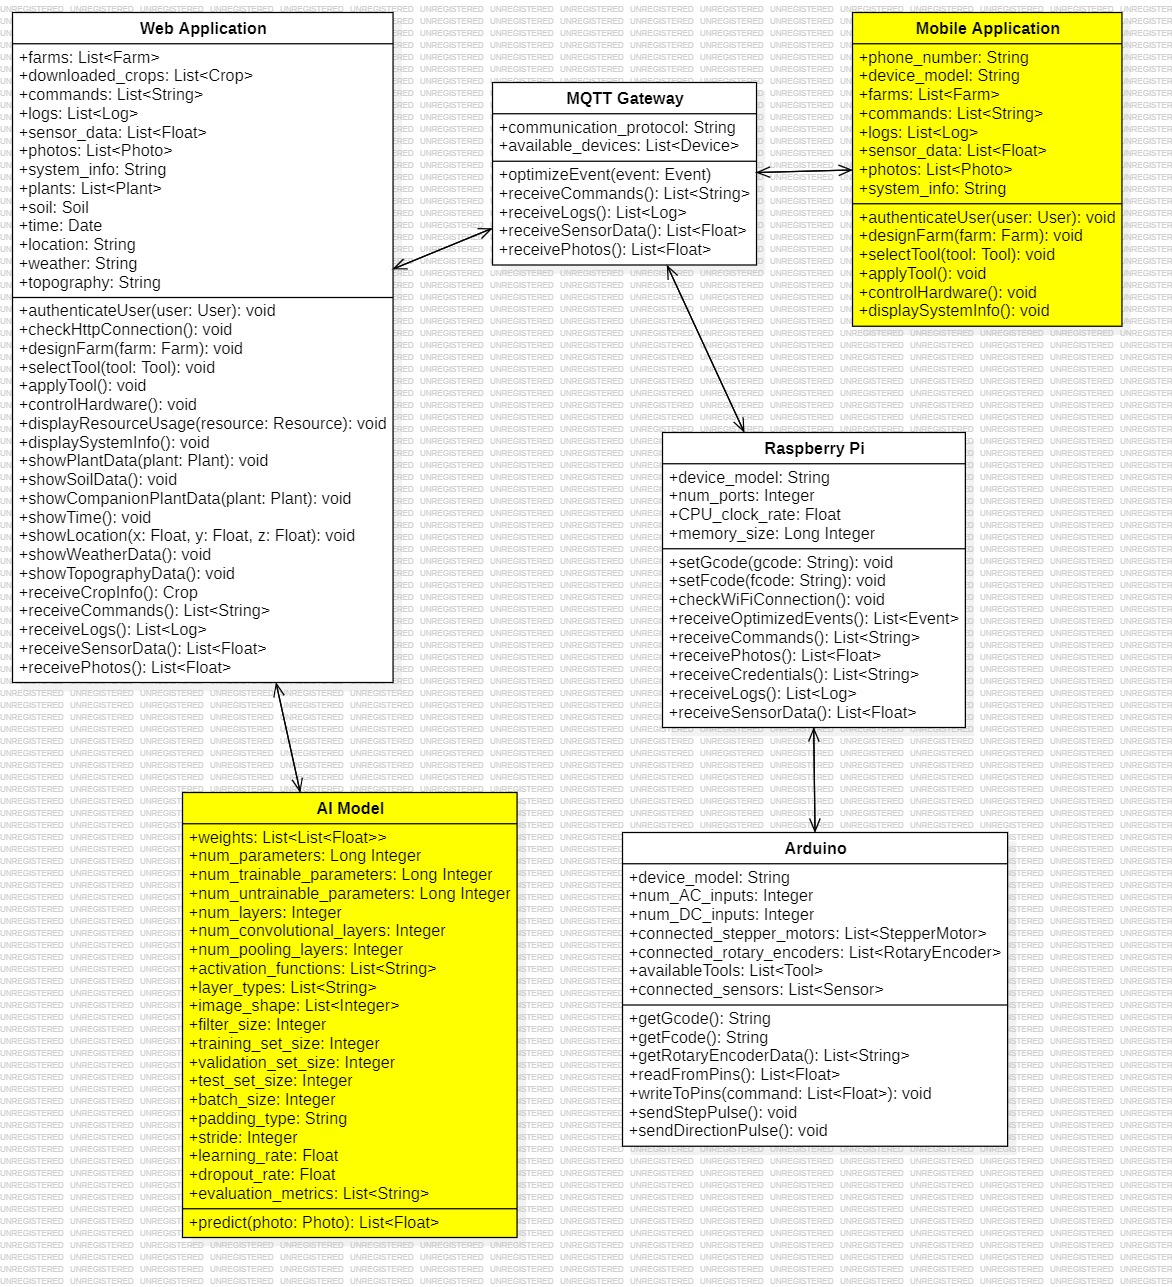
\includegraphics[width=0.9\linewidth]{Figures/improved_internal_interfaces.jpg}
    \caption{Internal Interfaces Class Diagram for the Improved System}
    \label{InternalImproved}
\end{figure}
\newpage
The integration of additional internal interfaces significantly enhances the functionality and responsiveness of the FarmBot system. The updated interfaces include new components Mobile Application and the AI Model interfaces:
\begin{itemize}
    \item \textbf{AI Model:}
        \begin{itemize}
            \item \textbf{weights:} The parameters of the neural network that are adjusted during the training process to minimize error.
            \item \textbf{num\_parameters:} Total number of parameters in the AI model.
            \item \textbf{num\_trainable\_parameters:} Parameters that can be adjusted during training to improve model accuracy.
            \item \textbf{num\_untrainable\_parameters:} Fixed parameters that do not change during the model's training.
            \item \textbf{num\_layers:} The total number of layers in the neural network.
            \item \textbf{num\_convolutional\_layers:} Number of layers that use convolutional neural network technology to process pixel data.
            \item \textbf{num\_pooling\_layers:} Layers designed to reduce the spatial size of convoluted features to decrease computational load and overfitting.
            \item \textbf{activation\_functions:} Functions like ReLU or sigmoid that introduce non-linear properties to the model.
            \item \textbf{layer\_types:} Types of layers used in the model, such as dense, dropout, or batch normalization.
            \item \textbf{image\_shape:} The dimensionality of input images that the model expects.
            \item \textbf{filter\_size:} The size of the filter used in convolutional layers.
            \item \textbf{training\_set\_size:} The number of samples in the training dataset.
            \item \textbf{validation\_set\_size:} The number of samples used to validate the model during training.
            \item \textbf{test\_set\_size:} The number of samples in the dataset used to test the model after training.
            \item \textbf{batch\_size:} Number of training examples utilized in one iteration.
            \item \textbf{padding\_type:} The type of padding used during convolution (e.g., 'same', 'valid').
            \item \textbf{stride:} The stride of the sliding window during convolution operations.
            \item \textbf{learning\_rate:} The step size at each iteration while moving toward a minimum of a loss function.
            \item \textbf{dropout\_rate:} Probability at which neurons are turned off randomly to prevent overfitting.
            \item \textbf{evaluation\_metric:} The metric used to measure the performance of the model during validation and testing.
            \item \textbf{predict}$()$: Function that applies the trained model to new data to generate predictions based on learned features.
        \end{itemize}
    \item \textbf{Mobile Application:}
        \begin{itemize}
            \item \textbf{phone\_number:} The contact number linked to the user account for identity verification and notifications.
            \item \textbf{device\_model:} Specifies the model of the mobile device using the application, useful for tailoring the app's performance to device capabilities.
            \item \textbf{farms:} A list of farms managed by the user, allowing easy switching and management of multiple locations.
            \item \textbf{commands:} Stores the list of commands that can be sent from the mobile device to the FarmBot, such as watering or moving.
            \item \textbf{logs:} Records of operations and system messages that help users track the activity and diagnose issues.
            \item \textbf{sensor\_data:} Real-time data collected from various sensors installed in FarmBot, providing insights into environmental conditions.
            \item \textbf{photos:} Images captured by FarmBot that are accessible through the mobile application for monitoring crop growth and health.
            \item \textbf{system\_info:} Information about the status and health of the FarmBot system, including software version and operational status.
            \item \textbf{authenticateUser}$()$: Function to verify the identity of the user, ensuring secure access to the app.
            \item \textbf{designFarm}$()$: Allows users to layout or modify the farm setup directly from their mobile device.
            \item \textbf{selectTool}$()$: Enables users to choose specific tools for tasks like planting or weeding via the app.
            \item \textbf{applyTool}$()$: Command to activate the selected tool on the FarmBot.
            \item \textbf{controlHardware}$()$: Direct control of the FarmBot hardware to execute tasks such as movement and adjustments.
            \item \textbf{displaySystemInfo}$()$: Displays detailed system status and diagnostics to the user on their mobile device.
        \end{itemize}
\end{itemize}

\newpage
\subsection{Interaction Patterns}
\begin{figure}[htbp]
    \centering
    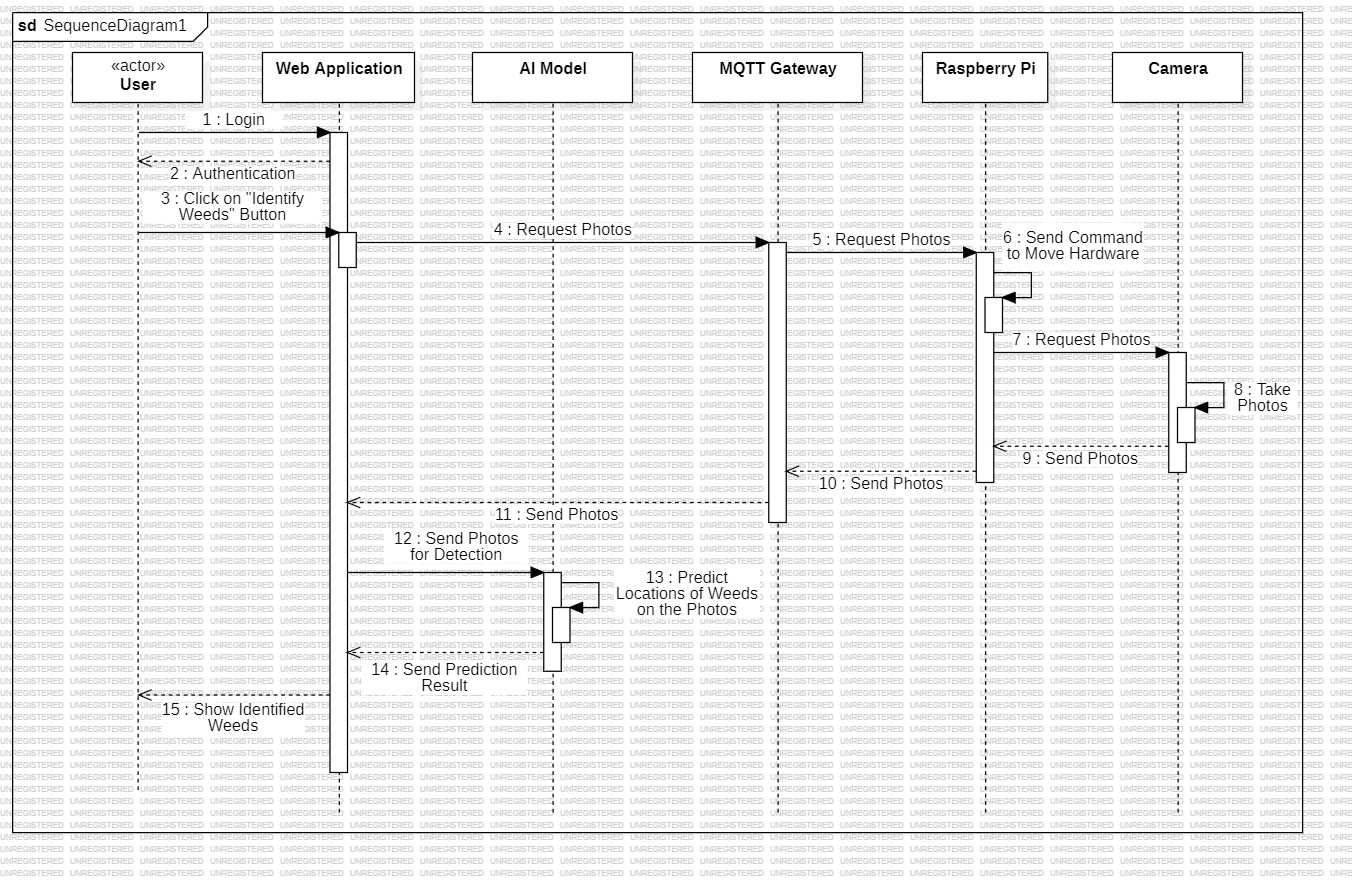
\includegraphics[width=1\linewidth]{Figures/sequence4.jpg}
    \caption{Sequence Diagram for "Identify Weeds" Interaction Pattern}
    \label{Sequence4}
\end{figure}
\newpage

\section{Information View}

\subsection{Stakeholders’ uses of this view}
The Information View is essential for stakeholders to comprehend and manage how data flows within FarmBot, especially with the addition of new features like AI-Driven Weed Identification and Disease Detection, Mobile Application, ForumBot, and the OpenWeather API. Here's how these new features impact data management:
\begin{itemize}
    \item \textbf{Hobbyist Gardeners and Professional Farmers:} These users look at the Information View to understand how data from the new OpenWeather API and AI-driven features are integrated and utilized. This view helps them see how weather forecasts affect FarmBot's operational decisions and how AI technologies improve weed and disease management, enhancing their farming practices with more precise data.
    \item \textbf{Educators:} They use the Information View to show students how data from external sources like weather APIs and community-generated content from ForumBot are managed and utilized by FarmBot. This helps illustrate the integration of real-world data into automated systems, providing a practical example of data-driven agriculture.
    \item \textbf{Researchers:} Interested in the data specifics for AI models and external data integration, researchers use this view to understand how FarmBot collects, stores, and analyzes data from the OpenWeather API and the AI systems for advanced agricultural studies.
    \item \textbf{Software Developers:} Developers rely on this view to grasp how new data streams from the mobile application and external interfaces like ForumBot and OpenWeather API are structured and stored within FarmBot’s database. This understanding is crucial for developing robust features that seamlessly integrate with FarmBot’s existing data architecture.
    \item \textbf{System Administrators:} System admins use the Information View to oversee the integration and management of new data sources and ensure the security and integrity of data flowing into FarmBot from the OpenWeather API and ForumBot. They monitor how data from these sources impacts system performance and troubleshoot any issues related to data handling.
    \item \textbf{Open-Source Contributors and Community Members:} These stakeholders examine the Information View to understand how new features like the mobile application and ForumBot alter data structures and flow within FarmBot. Insight into how these features collect and utilize data enables contributors to propose enhancements or develop additional functionalities that align with FarmBot’s data models.
\end{itemize}
The Information View helps stakeholders ensure that the integration and management of data from new internal and external features align with FarmBot's objectives of enhancing efficiency, sustainability, and educational value in automated farming.

\newpage
\subsection{Database Class Diagram}
\begin{figure}[htbp]
    \centering
    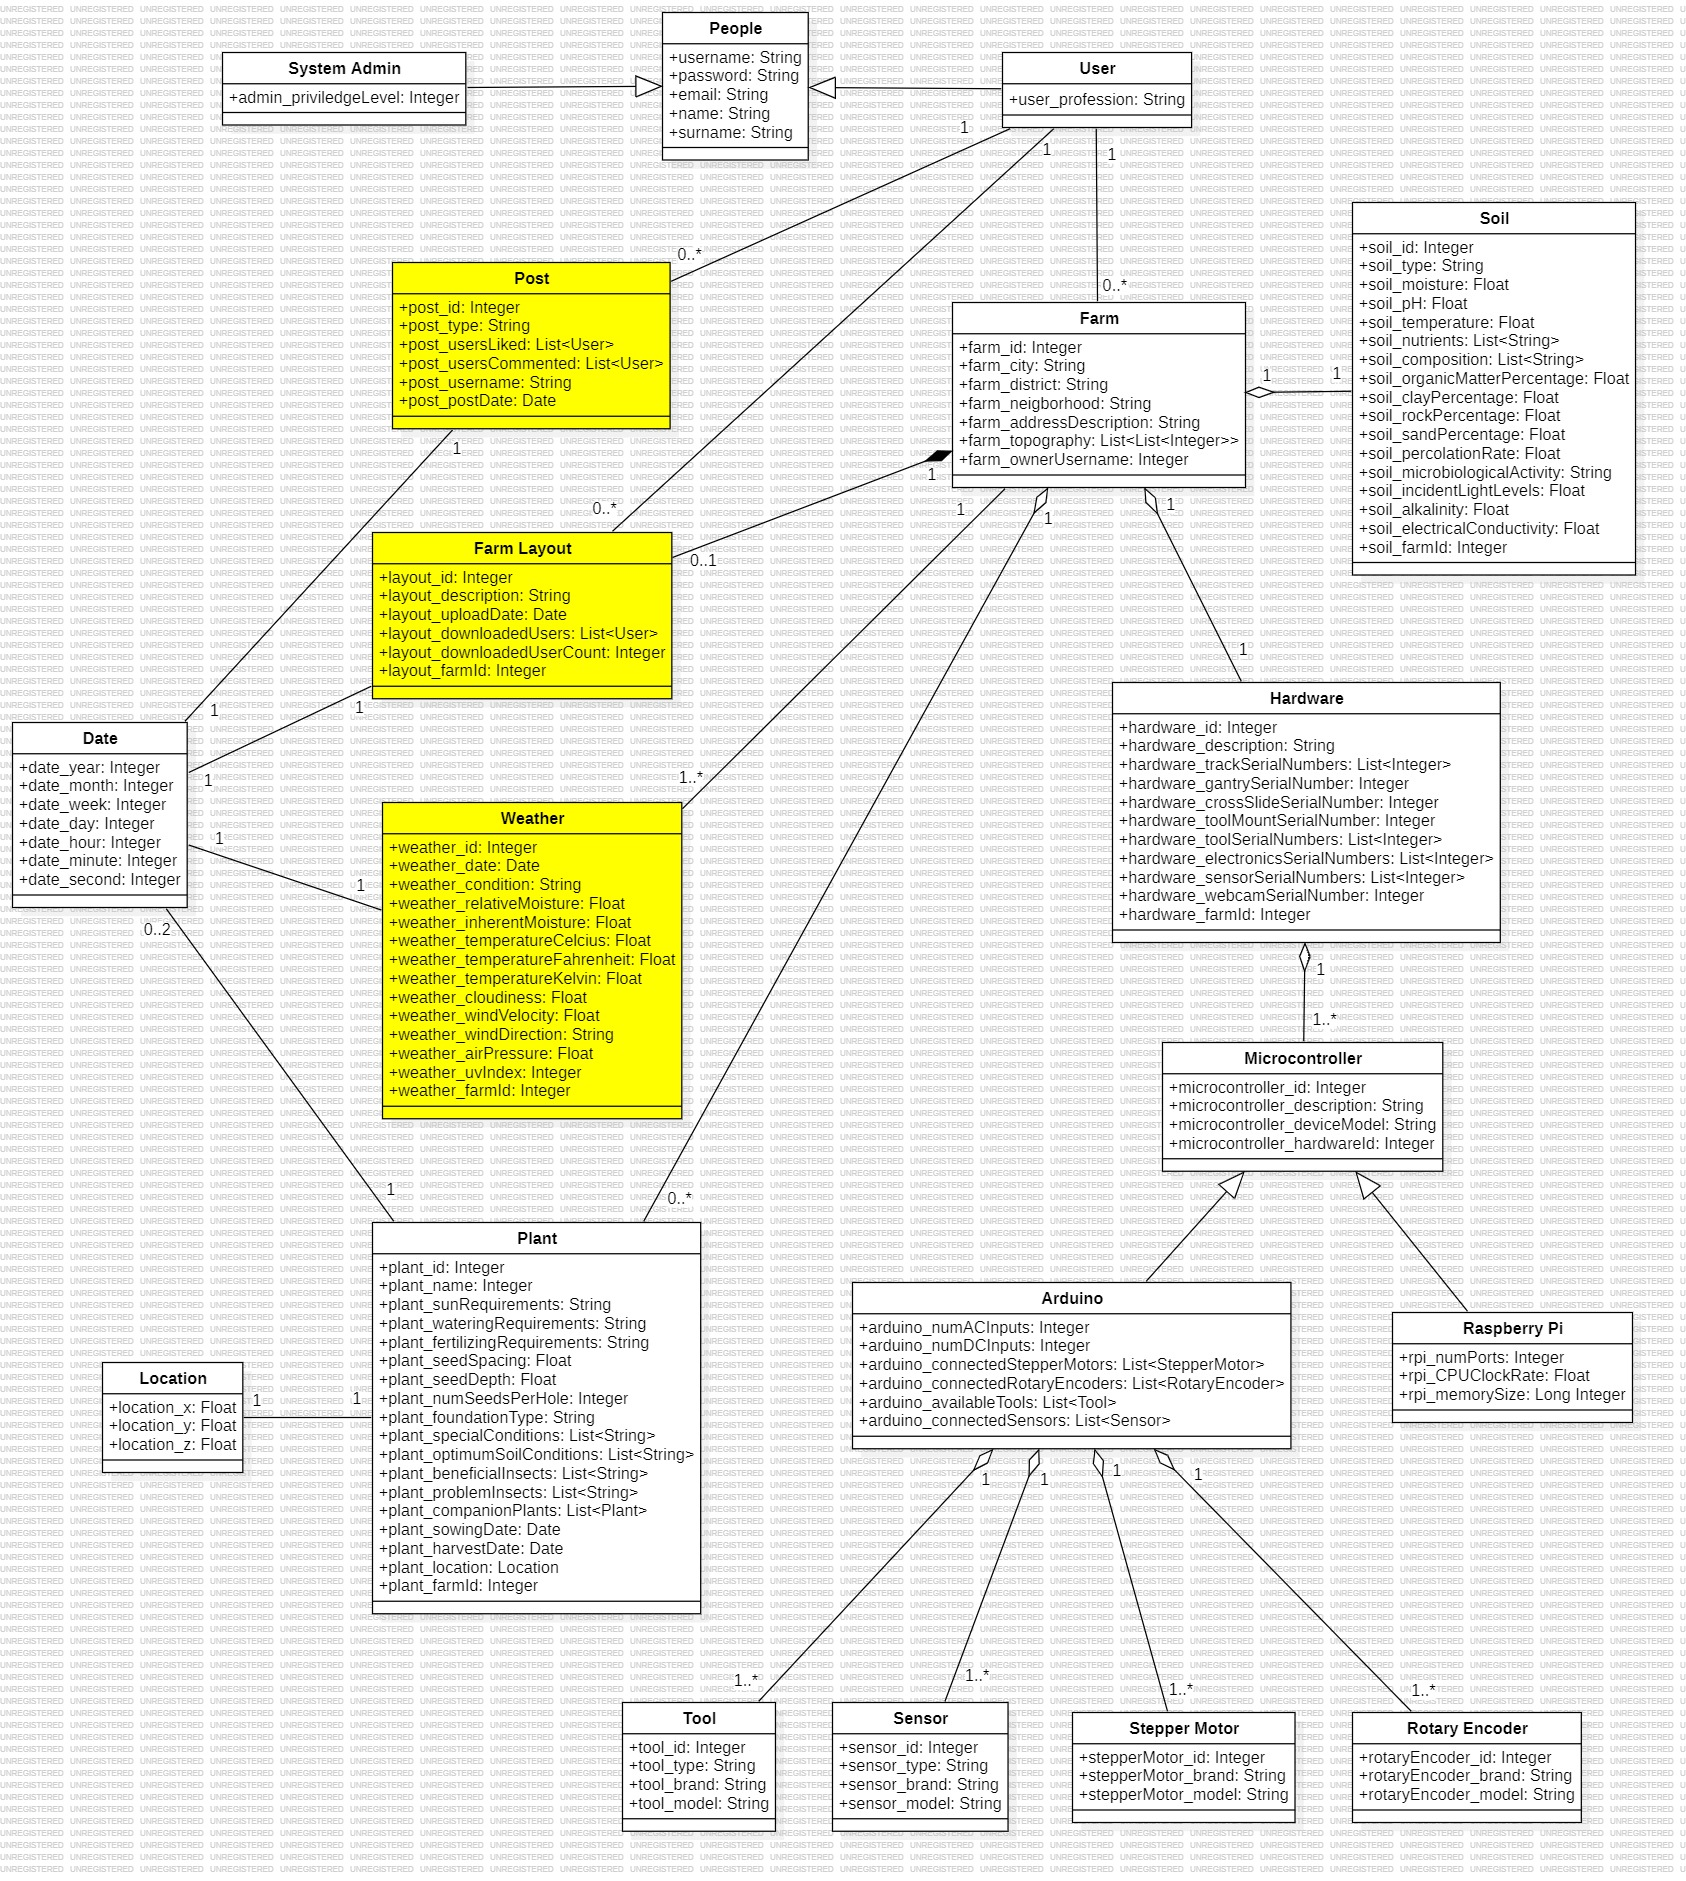
\includegraphics[width=0.9\linewidth]{Figures/improved_database_class_diagram.jpg}
    \caption{Database Class Diagram for the Improved System}
    \label{DatabaseImproved}
\end{figure}
\newpage

\subsection{Operations on Data}
\begin{longtblr}
[
    caption = {CRUD Operations for the Improved System},
    label = {CRUDImproved}
]
{
    colspec = {|X|X|},
    hlines
}
\textbf{Operation} & CRUD Operations  \\ \hline
\textbf{CreatePost} & {
    Create: Add a new post entry with details such as type, user comments, username, and post date.\\
    Read: -\\
    Update: -\\
    Delete: -
} \\ \hline
\textbf{ReadPost} & {
    Create: -\\
    Read: Retrieve details of a specific post by post ID.\\
    Update: -\\
    Delete: -
} \\ \hline
\textbf{SeeUsersLiked} & {
    Create: -\\
    Read: Show all the users that have liked a specific post.\\
    Update: -\\
    Delete: -
} \\ \hline
\textbf{SeeUsersCommented} & {
    Create: -\\
    Read: Show all the users that have commented on a specific post.\\
    Update: -\\
    Delete: -
} \\ \hline
\textbf{UpdatePost} & {
    Create: -\\
    Read: -\\
    Update: Update details of an existing post, such as type or comments.\\
    Delete: -
} \\ \hline
\textbf{DeletePost} & {
    Create: -\\
    Read: -\\
    Update: -\\
    Delete: Remove a post entry from the database.
} \\ \hline
\textbf{RegisterFarmLayout} & {
    Create: Register a new farm layout with description, upload date, and associated farm ID.\\
    Read: -\\
    Update: -\\
    Delete: -
} \\ \hline
\textbf{RetrieveFarmLayout} & {
    Create: -\\
    Read: Retrieve details of a specific farm layout by layout ID.\\
    Update: -\\
    Delete: -
} \\ \hline
\textbf{SeeUsersDownloaded} & {
    Create: -\\
    Read: Display usernames of users who have downloaded a specific farm layout.\\
    Update: -\\
    Delete: -
} \\ \hline
\textbf{UpdateFarmLayout} & {
    Create: -\\
    Read: -\\
    Update: Update description or download count of an existing farm layout.\\
    Delete: -     
} \\ \hline
\textbf{DeleteFarmLayout} & {
    Create: -\\
    Read: -\\
    Update: -\\
    Delete: Delete a specific farm layout from the database.
} \\ \hline
\textbf{LogWeatherData} & {
    Create: Log new weather data entry including date, condition, moisture levels, temperature, wind details, and UV index.\\
    Read: -\\
    Update: -\\
    Delete: -
} \\ \hline
\textbf{RetrieveWeatherData} & {
    Create: -\\
    Read: Retrieve weather data for a specific date or farm ID.\\
    Update: -\\
    Delete: -
} \\ \hline
\textbf{UpdateWeatherData} & {
    Create: -\\
    Read: -\\
    Update: Update existing weather data entries with new measurements or corrections.\\
    Delete: -
} \\ \hline
\textbf{DeleteWeatherData} & {
    Create: -\\
    Read: -\\
    Update: -\\
    Delete: Remove weather data for a specific date and farm from the database.
}
\end{longtblr}

\newpage
\section{Deployment View}

\subsection{Stakeholders’ uses of this view}
The Deployment View is essential for stakeholders to grasp how FarmBot's new and existing software components are distributed across its hardware and network infrastructure, particularly with the integration of AI-driven features, a mobile application, ForumBot, and the OpenWeather API:
\begin{itemize}
    \item \textbf{Hobbyist Gardeners and Professional Farmers:} They benefit from understanding that features like the mobile application and OpenWeather API enhance FarmBot's reliability and real-time operational capabilities, regardless of local network conditions.
    \item \textbf{Educators:} Use this view to show students the practical application of distributed computing, explaining how features like AI-driven weed identification are implemented across cloud and local devices.
    \item \textbf{Researchers:} Examine how the deployment of AI and external data integrations like the OpenWeather API impacts data accuracy and system responsiveness.
    \item \textbf{Software Developers:} Focus on optimizing code for diverse environments, ensuring efficient operation of features across cloud platforms and mobile devices.
    \item \textbf{System Administrators:} Manage the integration and maintenance of new features, ensuring all components are properly configured for efficient operation.
    \item \textbf{Open-Source Contributors and Community Members:} Refer to this view to ensure their contributions integrate seamlessly with FarmBot’s multi-layered architecture, enhancing functionality and compatibility.
\end{itemize}
This Deployment View helps stakeholders ensure that FarmBot's system is effectively scaled and robust, ready to meet operational demands and maintain high performance.

\newpage
\subsection{Deployment Diagram}
\begin{figure}[htbp]
    \centering
    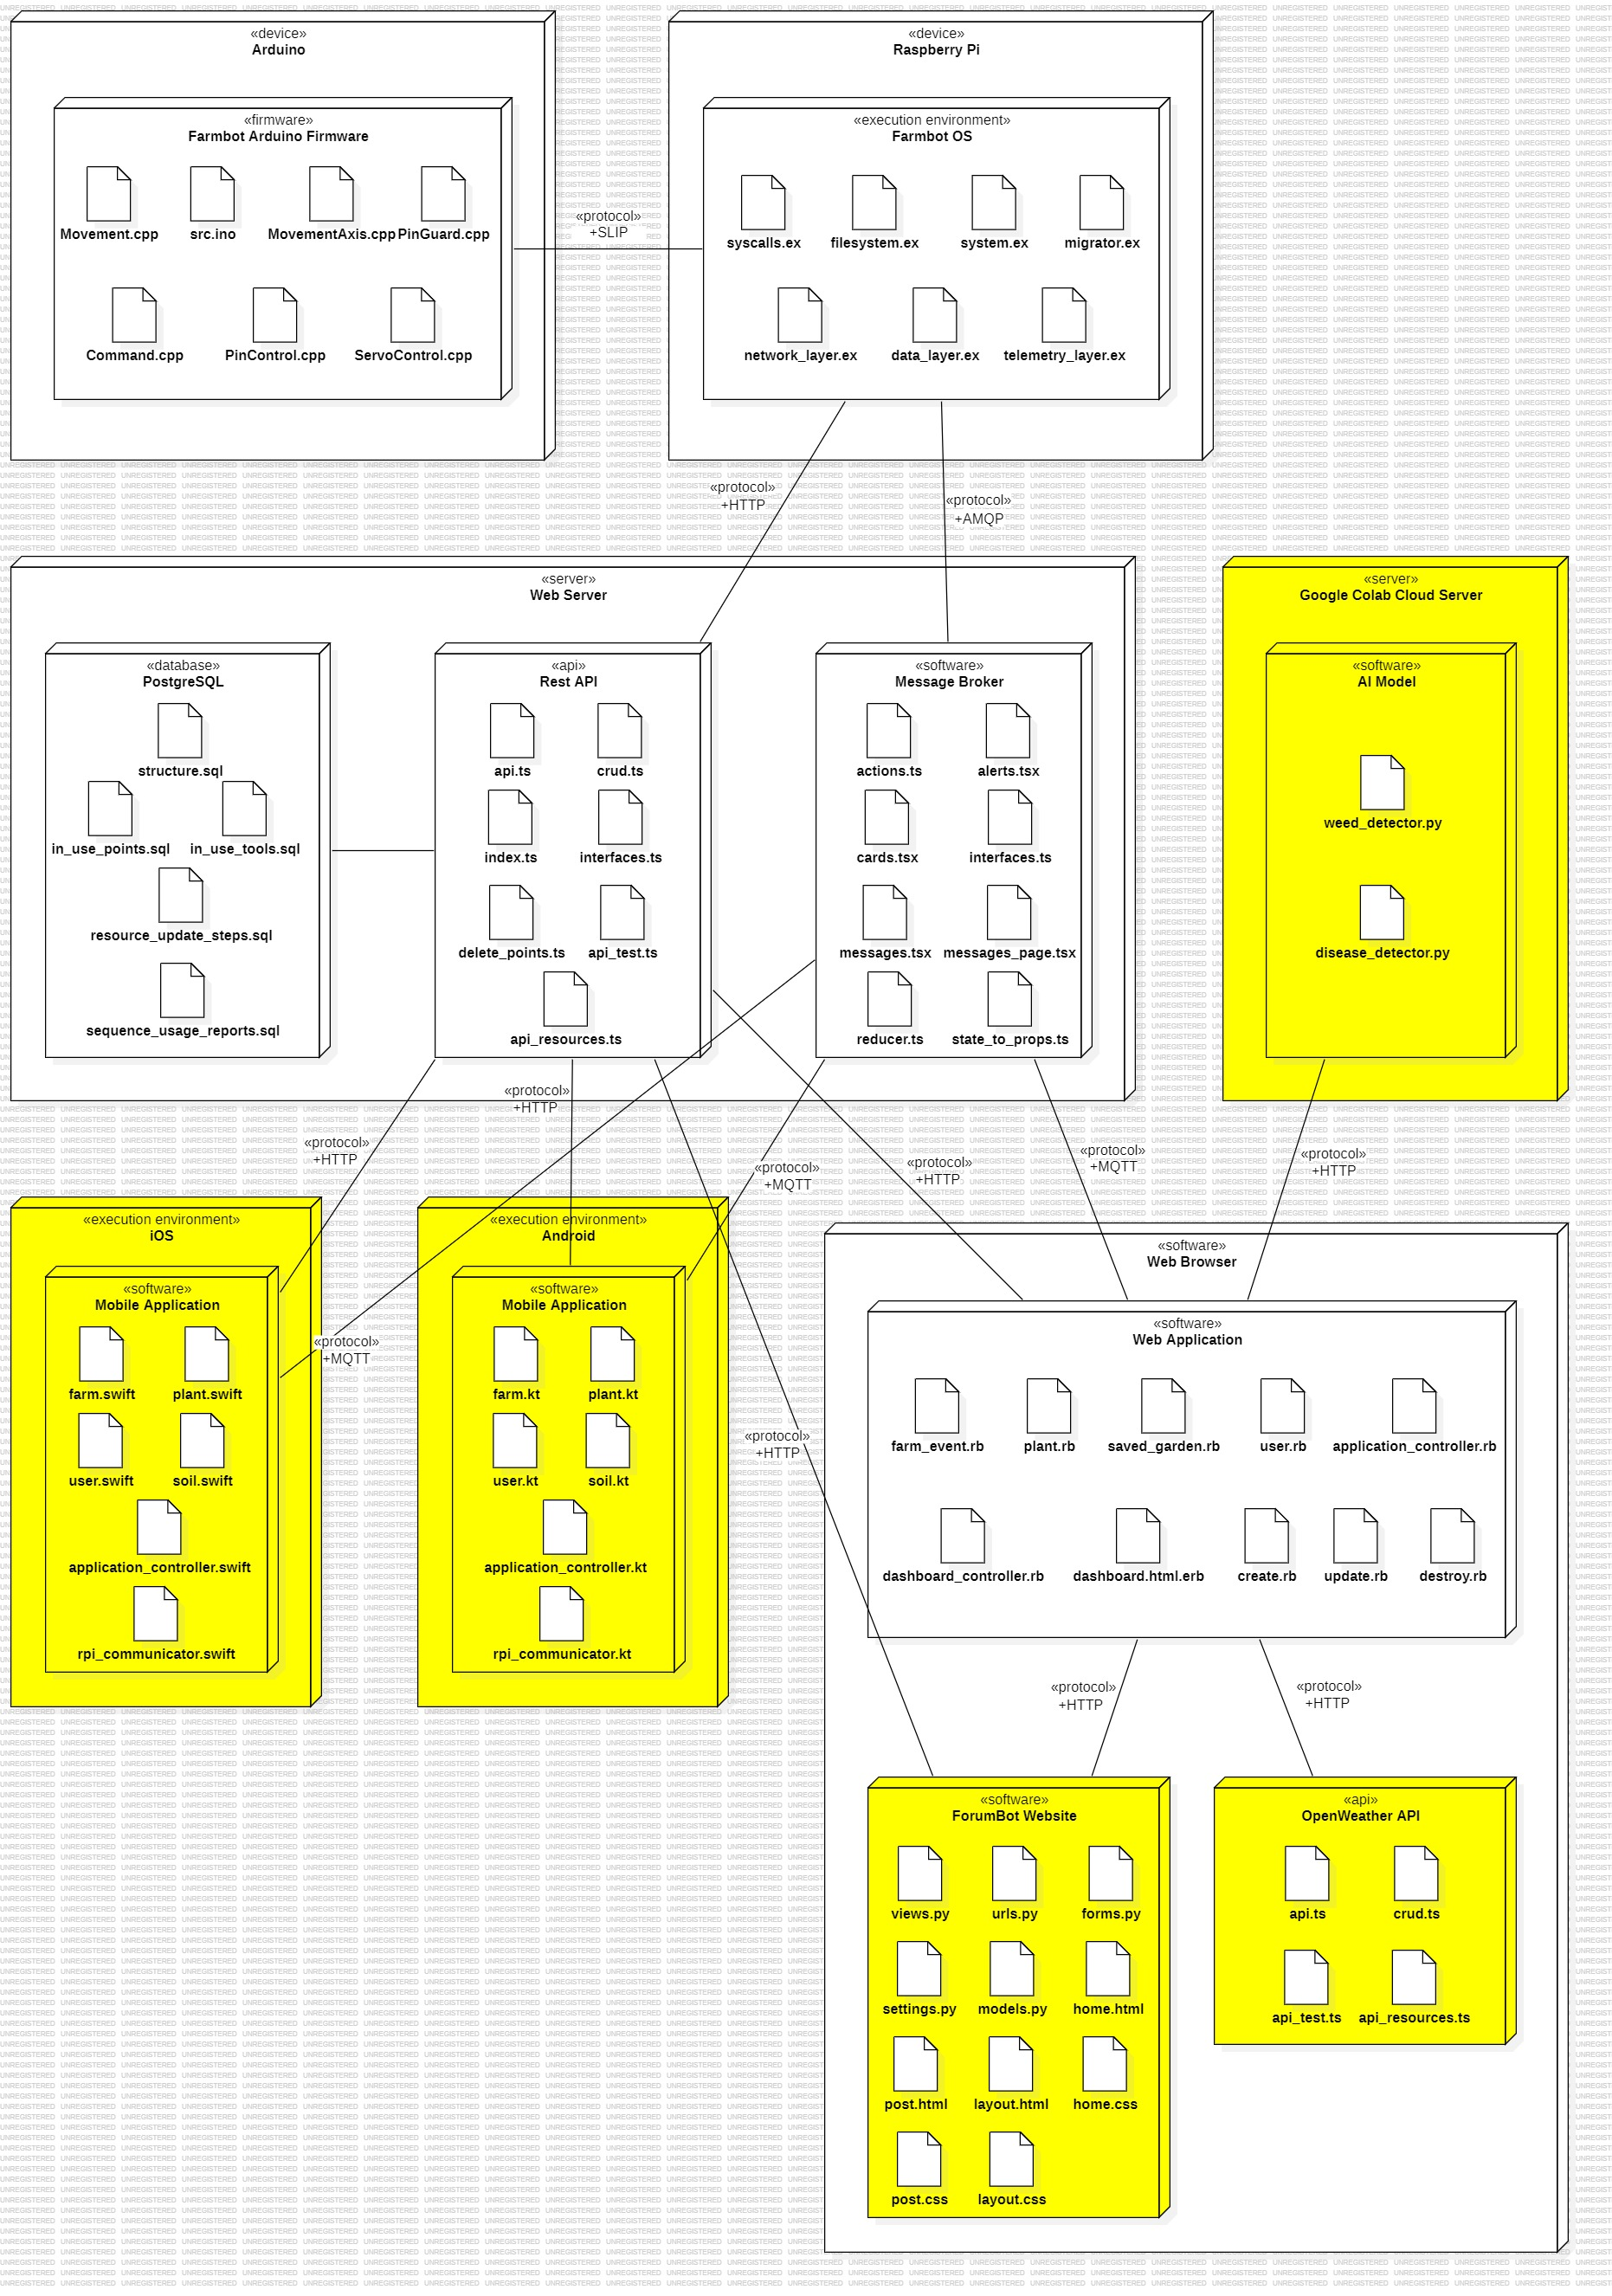
\includegraphics[width=0.7\linewidth]{Figures/improved_deployment_diagram.jpg}
    \caption{Deployment Diagram for the Improved System}
    \label{DeploymentImproved}
\end{figure}
\newpage
The enhanced deployment diagram for FarmBot integrates several new components and services, reflecting the system's evolution and expansion to accommodate advanced functionalities and broader connectivity. These additions represent significant enhancements to the system’s capabilities:
\begin{itemize}
    \item \textbf{Google Colab Cloud Server:} This server hosts the AI Model, comprising scripts like weed\_detector.py and disease\_detector.py. These Python scripts leverage machine learning algorithms to identify weeds and detect plant diseases, enhancing FarmBot's autonomous capabilities. The deployment on Google's Colab platform allows for computational resources and scalability.
    \item \textbf{Mobile Applications for iOS and Android:} The Mobile Application on both iOS and Android platforms, illustrated separately for each operating system, features software components like farm.swift, plant.kt, and user.swift/user.kt. These components are responsible for providing mobile users with real-time access to FarmBot's functionalities, including farm management, plant monitoring, and user account management. The deployment on mobile platforms enhances user accessibility and interaction, utilizing MQTT for real-time communication.
    \item \textbf{ForumBot Website:} Deployed within the Web Browser, the ForumBot Website includes files such as views.py, urls.py, and forms.py which handle the dynamic content generation, URL routing, and form management for user interactions. This platform serves as a community hub where users can share insights, discuss various topics, and exchange farming strategies, fostering a collaborative environment.
    \item \textbf{OpenWeather API:} Also within the Web Browser, the OpenWeather API, with files like api.ts and crud.ts, allows FarmBot to retrieve real-time weather data crucial for farm management decisions. The integration of this API facilitates automated responses to weather changes, optimizing watering schedules and protecting plants from adverse conditions.
\end{itemize}
These new features are seamlessly integrated into FarmBot's existing deployment framework, ensuring robust performance and enhancing user experience. The use of HTTP/HTTPS for secure web interactions and MQTT for mobile and IoT communications reflects a well-structured deployment strategy that supports both scalability and reliability.

\newpage
\section{Design Rationale}
\textbf{Design Rationale for Context View}\\
Integrating the OpenWeather API and introducing ForumBot into the Context View enhances FarmBot's environmental responsiveness and community interaction. The OpenWeather API allows real-time weather data to directly inform farming decisions, improving irrigation and pest management. ForumBot fosters community engagement, enabling users to share insights and strategies, supporting the open-source philosophy and broadening the collaborative knowledge base.\\\\
\textbf{Design Rationale for Functional View}\\
The addition of AI-Driven Weed Identification and Disease Detection and a Mobile Application in the Functional View enhances FarmBot’s operational efficiency and user interaction. AI features automate plant health management, reducing the need for manual monitoring, while the mobile app increases accessibility, allowing users to manage and monitor FarmBot remotely.\\\\
\textbf{Design Rationale for Information View}\\
Updating the Information View to include data flows from the OpenWeather API and ForumBot ensures FarmBot can utilize real-time environmental data and user-generated content effectively. This approach enhances FarmBot’s adaptability and decision-making processes, maintaining data integrity and scalability.\\\\
\textbf{Design Rationale for Deployment View}\\
The new deployment of cloud-based services for the OpenWeather API and ForumBot on scalable cloud infrastructure ensures high system responsiveness and adaptability. This deployment supports dynamic adjustments to environmental changes and user interactions, maintaining FarmBot’s performance and reliability.